\documentclass[journal=asbcd6,manuscript=article,keywords]{achemso}

\usepackage{graphicx}
\usepackage{amsmath}
\usepackage{subcaption}
\usepackage{array}
\usepackage{amssymb}
\usepackage{siunitx}
\usepackage{url}
\usepackage{longtable}
\usepackage{booktabs}
\usepackage{tikz}

\usetikzlibrary{positioning, arrows.meta}

\title{Reservoir Computing with Quorum-Sensing Genetic Oscillators for Biosignal Classification}

\author{James Newsome}
\affiliation[Newcastle]{School of Computing, Newcastle University, Newcastle upon Tyne, NE1 7RU, United Kingdom}
\email{james.newsome02@gmail.com}

\author{Gizem Buldum}
\affiliation[Newcastle]{School of Computing, Newcastle University, Newcastle upon Tyne, NE1 7RU, United Kingdom}

\author{Tim Rudge}
\affiliation[Newcastle]{School of Computing, Newcastle University, Newcastle upon Tyne, NE1 7RU, United Kingdom}

\keywords{Reservoir Computing, Genetic Oscillators, Biosignal Classification, Echo State Network, Synthetic Biology, Arrhythmia Detection}

\begin{document}

\begin{abstract}
Reservoir computing offers a compelling framework for biological computation, as complex temporal processing can be achieved without training internal network dynamics. Here, we present a biologically grounded reservoir computing architecture composed of coupled quorum-sensing genetic oscillators. Each reservoir node simulates a two-gene LuxI/AiiA circuit with a delayed activator--inhibitor feedback architecture mediated by intracellular and extracellular acyl-homoserine lactone (AHL), producing rich oscillatory dynamics. Spatial coupling between nodes is implemented using a distance-based interaction kernel calibrated to experimentally observed quorum-sensing ranges. We demonstrate the computational capability of this system by performing multi-class classification of single-lead electrocardiogram (ECG) signals, achieving a macro F1-score of $0.890 \pm 0.007$ on balanced five-class arrhythmia classification using five-fold cross-validation. Performance increases to $0.920 \pm 0.005$ under clinically realistic class imbalance, and $0.961 \pm 0.002$ for binary arrhythmia detection. The ECG task serves as a standardized benchmark for temporal computational capability rather than a clinical application; the goal is to demonstrate that complex sequential classification is achievable using biological dynamics alone. Our results establish quorum-sensing oscillator networks as a viable substrate for reservoir computing, and the systematic optimization yields quantitative design specifications---including optimal reservoir size, coupling range, and input scaling---to guide future wet-lab implementations.
\end{abstract}

% ---------- Main Content ----------

\section{Introduction}

Synthetic biology has produced a range of engineered genetic circuits capable of computation, including switches, amplifiers, memory elements, and oscillators~\cite{Green2014,Bonnet2013,Gardner2000,Elowitz2000,Uriu2016}. Among these, the quorum-sensing oscillator of Danino et al.~\cite{Danino2010} was a landmark achievement, demonstrating synchronized, population-level oscillations across \textit{E. coli} colonies. Such oscillators generate structured, time-varying gene expression patterns through delayed feedback regulation~\cite{Goldbeter2012, Uriu2016}. In parallel, DNA-based reservoir computing was first demonstrated in 2013, achieving 90\% accuracy on a temporal benchmark~\cite{Goudarzi2013}, and has since been extended to DNA oscillator reservoirs~\cite{Liu2022} and cascaded DNA memristors~\cite{Liu2024}. These molecular approaches operate in cell-free nucleic-acid reaction networks with abstract chemical kinetics~\cite{Goudarzi2013,Liu2022}. Most recently, Ahavi et al.~\cite{Ahavi2024} demonstrated reservoir computing with living bacterial populations. Our work differs from both lines by modeling gene expression dynamics in living cells through experimentally validated delay differential equations and spatially coupled quorum sensing, bridging the gap between in vitro molecular computing and in vivo biological substrates.

Reservoir computing (RC), formalized in the echo-state approach to recurrent neural networks (RNNs), offers a simple yet powerful paradigm for temporal pattern recognition~\cite{Jaeger2001,Zhang2023}. An RC system comprises an input layer, a high-dimensional fixed dynamical reservoir, and a trainable readout layer~\cite{Jaeger2001,Nakajima2020}. The reservoir's internal weights are fixed upon initialization, allowing the input signals to easily perturb its dynamics, producing diverse nonlinear responses with fading memory of past inputs~\cite{Tanaka2019}. This separation of dynamic representation and training reduces the computational cost and risk of overfitting compared to fully trained deep networks, making RC attractive when a lightweight readout is desirable and encouraging physical reservoir implementations~\cite{Konkoli2018,Wang2024}.

Biological systems, such as microbial cultures or synthetic gene circuits, can be viewed as natural computing reservoirs where external chemical or environmental stimuli influence the reservoir by modulating quorum-sensing pathways and diffusive signaling~\cite{Dambre2012}. For instance, \textit{E. coli} populations can coordinate gene expression via acyl-homoserine lactone (AHL) signaling molecules~\cite{Reading2006}, providing a mechanism for both intra- and inter-node coupling in a biological reservoir; with delays, nonlinearity, and spatial coupling emerging naturally from gene regulation and molecular transport. For example, in Prindle's arsenic biosensor~\cite{Prindle2011}, arsenite modulates the period of synchronized quorum-sensing oscillations across an array of thousands of \textit{E. coli} biopixels, with inter-biopixel coupling achieved through gas-phase H$_2$O$_2$ redox signaling rather than AHL alone. The oscillatory period, read out via sfGFP fluorescence, serves as the biosensor output. To date, RC has been applied to various physical and simulated substrates~\cite{Tanaka2019,Wang2024}, but integrating biologically realistic genetic oscillator models into RC frameworks remains mostly unexplored, particularly those incorporating experimentally calibrated delays, diffusion ranges, and spatial coupling. Such integration could provide a biologically plausible computational architecture, potentially translatable to the wet-lab. Moreover, modeling these dynamics in silico offers a testbed for synthetic gene circuits before costly experimental implementation.

In this work, we implement a gene-based reservoir computer, utilizing the open-source RC framework “reservoirpy”~\cite{Trouvain2020}. Each reservoir node simulates a quorum-sensing genetic bio-pixel modeled by delay differential equations capturing transcriptional, translational, and signaling delays; with parameters taken from the design of a genetic clock by Danino et al.~\cite{Danino2010}. Coupling between oscillators allows the network to exhibit complex spatiotemporal dynamics in response to input perturbations. These dynamics project incoming signals into a high-dimensional space, enabling a simple readout classifier to discriminate between signal classes~\cite{Maass2002}. As a benchmark, we apply this architecture to the clinically relevant task of electrocardiogram (ECG) arrhythmia classification. ECG signals are rich in temporal structure~\cite{Rafie2021}, making them ideal for evaluating the reservoir’s ability to capture and transform temporal dependencies. Using the MIT-BIH Arrhythmia Database~\cite{Moody2001}, with preprocessing from Kachuee et al.~\cite{Kachuee2018}, our model achieved non-trivial performance on balanced and unbalanced classification tasks.

By modeling coupled quorum-sensing genetic oscillators within a reservoir computing framework, this work introduces a biologically grounded dynamical substrate for temporal information processing. Although computationally more complex than conventional neuronal reservoirs, the architecture captures key features of gene regulatory systems, including delays, nonlinearity, and spatial coupling, that are difficult to represent in abstract models. This approach enables systematic exploration of how genetic circuit dynamics can be harnessed for computation, while remaining compatible with established reservoir computing workflows. We demonstrate the feasibility of this paradigm on a real-world biomedical signal classification task and provide a flexible computational framework to support future studies in biologically inspired computing, biosensing, and synthetic gene circuit design.

\section{Results}

We first report the headline balanced, unbalanced, and binary classification results, then compare topology and readout choices, and finally summarize the optimization and ablation studies that support the mechanistic interpretation. The reservoir was selected through a four-phase optimization workflow: Phase~1 screened individual parameter groups, Phase~2 jointly refined the full configuration, Phase~3 evaluated alternative task settings, and Phase~4 optimized the readout on frozen reservoir states. Detailed study names, search ranges, and per-study diagnostics are reported in the Supporting Information.

\subsection{Balanced Five-Class ECG Classification}

Using the optimized reservoir configuration ($N = 1000$ quorum-sensing oscillator nodes, distance-based topology, $K$-nearest neighbors readout with $k = 4$, distance-weighted), we evaluated classification performance on the balanced five-class ECG arrhythmia task using five-fold stratified cross-validation. The model achieved a macro F1-score of $0.890 \pm 0.007$, with accuracy $0.890$, Matthews correlation coefficient (MCC) $0.863$, and Cohen's $\kappa = 0.862$ (Table~\ref{tab:balanced-metrics}). As the reservoir configuration was chosen using a single data fold, these standard deviations reflect only fold-to-fold variation in the final evaluation and underestimate the total uncertainty.

\begin{table}
\centering
\caption{Per-class classification metrics for the balanced five-class task (mean $\pm$ std across five folds, $N = 1000$, KNN $k = 4$, distance-weighted).}\label{tab:balanced-metrics}
\small
\begin{tabular}{lcccc}
\toprule
Class & Precision & Recall & F1-score & Support \\
\midrule
Normal (N)     & $0.775 \pm 0.020$ & $0.883 \pm 0.017$ & $0.825 \pm 0.016$ & ${\sim}161$ \\
Supraventricular (S) & $0.881 \pm 0.016$ & $0.836 \pm 0.023$ & $0.857 \pm 0.018$ & ${\sim}161$ \\
Ventricular (V) & $0.934 \pm 0.013$ & $0.854 \pm 0.024$ & $0.892 \pm 0.013$ & ${\sim}161$ \\
Fusion (F)     & $0.913 \pm 0.021$ & $0.915 \pm 0.012$ & $0.914 \pm 0.012$ & ${\sim}161$ \\
Unknown (Q)    & $0.967 \pm 0.011$ & $0.961 \pm 0.011$ & $0.964 \pm 0.009$ & ${\sim}161$ \\
\midrule
Macro avg.     &       &        & $0.890 \pm 0.007$ & 803 \\
\bottomrule
\end{tabular}
\end{table}

Performance varied across arrhythmia classes: the Unknown (Q) class was classified most reliably ($F_1 = 0.964$), while Normal (N) heartbeats were the most frequently misclassified ($F_1 = 0.825$), primarily through confusion with Supraventricular (S) beats, consistent with their morphological similarity (Figure~\ref{fig:five-class-results}a). All five arrhythmia classes exceeded $F_1 = 0.82$, with low inter-fold variance ($\sigma \leq 0.018$), indicating stable generalization across data partitions. This pattern is consistent with the class-average waveforms in Figure~\ref{fig:dataset-figure}a: N and S share a narrow QRS complex and comparatively subtle differences in the surrounding morphology, whereas Q has the most visually distinct waveform and is therefore separated reliably even by a simple local readout on the reservoir state space.

\begin{figure}
    \centering
    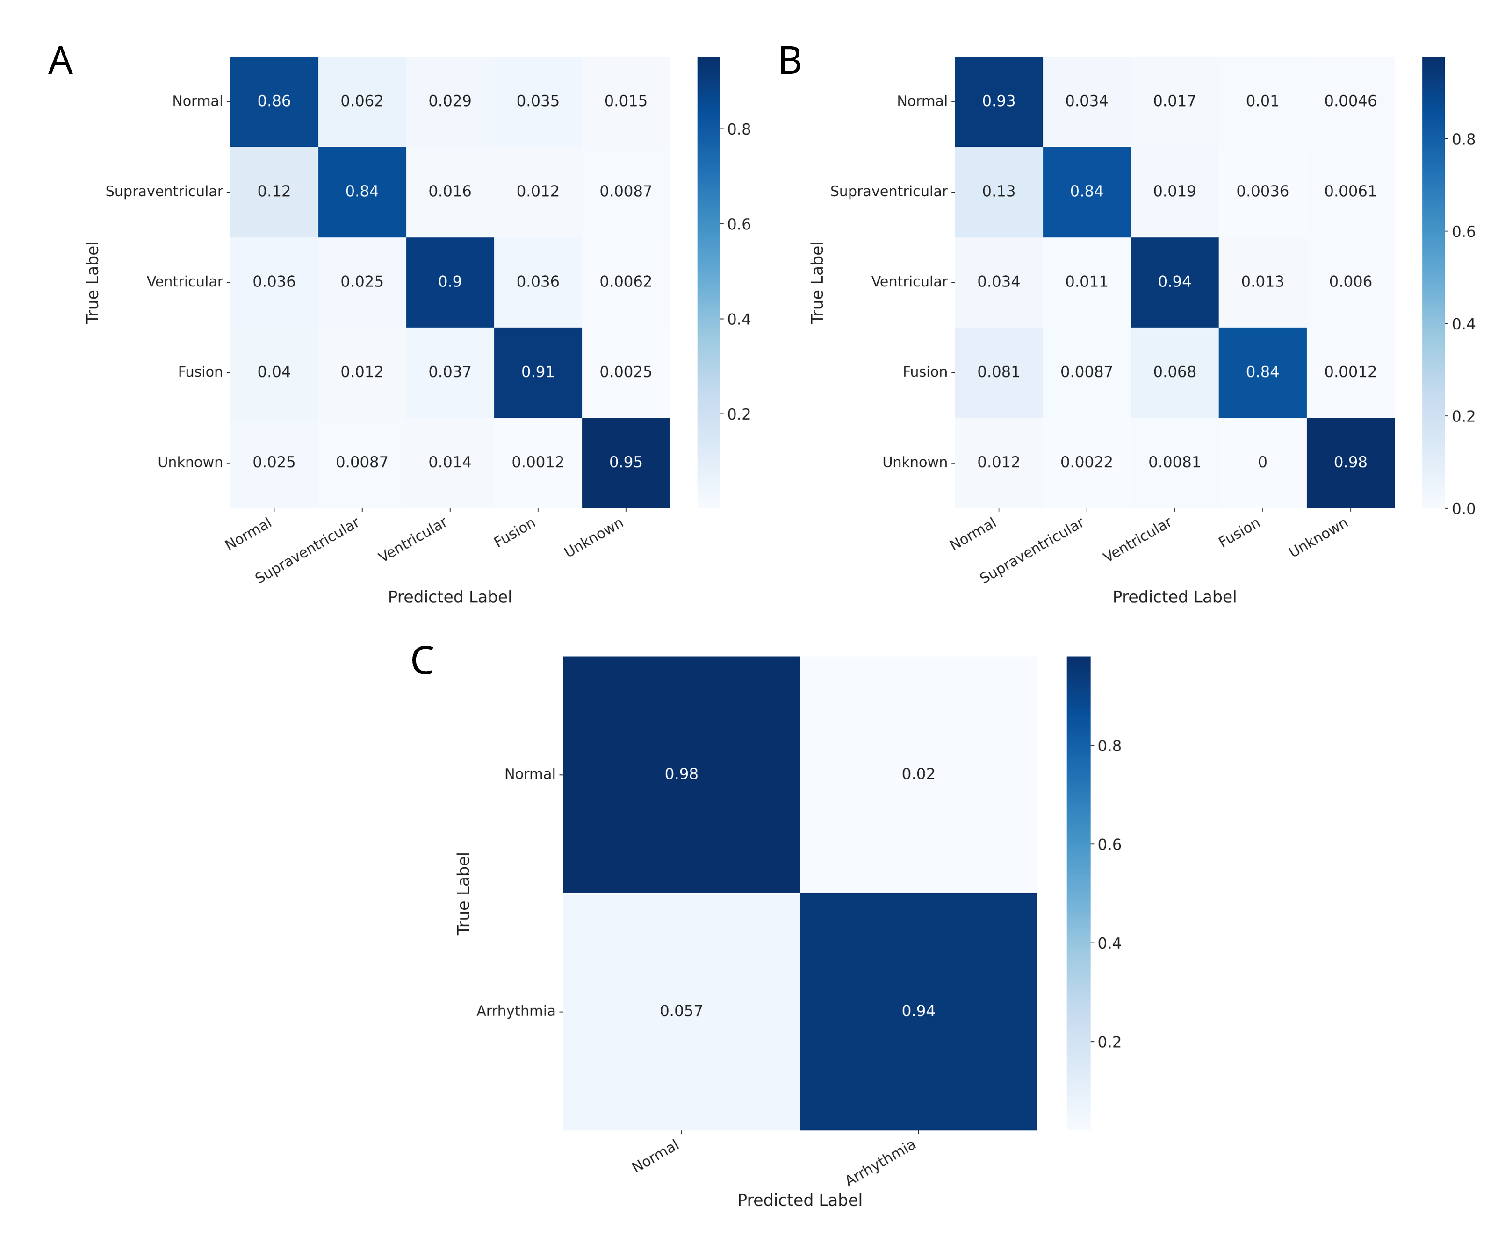
\includegraphics[width=\textwidth]{figures/article/headline-conf-matrices.pdf}
    \caption{Headline classification confusion matrices ($N = 1000$), aggregated across five folds and normalized by row. (a)~Balanced five-class configuration (KNN $k = 4$, distance-weighted). Normal (N) and Supraventricular (S) show the highest mutual confusion. (b)~Unbalanced five-class configuration (KNN $k = 1$, uniform). Additional majority-class training data reduces N--S confusion. (c)~Binary classification (Random Forest), where Normal retains the higher recall and Arrhythmia the higher precision. Because the matrices pool predictions across all folds before row normalization, the diagonal entries are not numerically identical to the mean per-fold recalls reported in Table~\ref{tab:balanced-metrics} and Table~\ref{tab:binary-metrics}.}\label{fig:five-class-results}
\end{figure}

Kachuee et al.~\cite{Kachuee2018} reported 93.4\% accuracy on the same MIT-BIH release using a deep convolutional neural network; however, their evaluation used the original highly imbalanced five-class setting, in which overall accuracy is dominated by the majority Normal class, so a direct comparison is not appropriate. Our balanced evaluation protocol (803 samples per class) provides a more stringent assessment of per-class discrimination. The genetic oscillator reservoir achieves competitive multi-class classification entirely through fixed biological dynamics and a simple readout, without the representational capacity of trainable deep layers.

\subsection{Effect of Class Imbalance and Dataset Size}

To examine how classification scales with dataset size and class distribution, we performed a grid search over the maximum samples per class, scaling the cap from $1\times$ (803) to $5\times$ (4015). Each class contributes up to the cap or its available count, whichever is smaller; consequently, the Fusion class (803 total) is the smallest contributor throughout, while Supraventricular reaches its natural limit of $2{,}779$ at $4\times$ and above. The effective CV pool size includes an additional 800-instance balanced reserve set (see Methods). Stratified five-fold cross-validation then preserves the resulting unequal class proportions in each fold's training and test subsets. This simulates the realistic clinical scenario in which normal heartbeats far outnumber pathological events. The macro F1-score increased monotonically from $0.882$ at $1\times$ to $0.920$ at $5\times$ (Table~\ref{tab:imbalance-scaling}), indicating that the reservoir benefits from additional training examples. Note that this imbalance study uses KNN $k = 1$ (uniform) throughout for comparability across all imbalance levels; the headline balanced result of $0.890$ (Table~\ref{tab:balanced-metrics}) uses the Phase~4-optimal $k = 4$ (distance-weighted) readout.

\begin{table}
\centering
\caption{Macro F1-score as a function of the per-class training cap. Each class contributes up to the cap or its available count. The CV Pool Size reflects the capped pool plus the fixed balanced 800-beat reserve set (160 per class) generated by the preprocessing pipeline. For example, at $1\times$ the reserve removes 160 from each class before capping; Fusion (803 total) then contributes only $803 - 160 = 643$ to the training cap, while the other four classes contribute the full cap of 803, giving a pool of $4 \times (803 + 160) + (643 + 160) = 4{,}655$. Values are from five-fold stratified cross-validation using $N = 1000$, KNN $k = 1$.}
\label{tab:imbalance-scaling}
\small
\begin{tabular}{cccc}
\toprule
Multiplier & Max per Class & CV Pool Size & Macro F1 \\
\midrule
$1\times$ & 803 & 4\,655 & 0.882 \\
$2\times$ & 1\,606 & 7\,867 & 0.894 \\
$3\times$ & 2\,409 & 11\,079 & 0.908 \\
$4\times$ & 3\,212 & 13\,698 & 0.913 \\
$5\times$ & 4\,015 & 16\,107 & 0.920 \\
\bottomrule
\end{tabular}
\end{table}

Using the full $5\times$ unbalanced configuration with five-fold cross-validation, the model achieved higher aggregate performance than in the strictly balanced setting. Weighted averages improve more strongly than macro averages because the additional data primarily benefits the already frequent Normal class, whereas the minority Fusion class remains the most fragile category. Figure~\ref{fig:five-class-results}b shows that the dominant effect of additional majority-class data is a reduction in Normal--Supraventricular confusion rather than a uniform improvement across all classes. For this reason, macro F1 is the primary headline metric in this work; per-class precision, recall, and F1-score for the unbalanced task are reported in the Supporting Information (Table~S17).

\subsection{Binary Arrhythmia Detection}

For a clinically oriented screening task, we merged all non-Normal classes into a single Arrhythmia category and performed binary classification using the same reservoir configuration. Both classes were balanced to the smaller merged class size ($18{,}857$ instances per class; $37{,}714$ total CV pool), yielding approximately $30{,}172$ training and $7{,}542$ test instances per fold in total, or about $15{,}086$ training and $3{,}771$ test instances per class. The model achieved a macro F1-score of $0.961 \pm 0.002$, with accuracy $0.961$, MCC $= 0.923$, and Cohen's $\kappa = 0.922$ (Table~\ref{tab:binary-metrics}), with the Arrhythmia class achieving higher precision ($0.979$) and the Normal class achieving higher recall ($0.980$). Readout algorithm selection (Phase~4) was performed on a $4{,}015$-instance subset for parity with the five-class studies, identifying random forest as the best binary classifier; the headline result was then obtained by retraining with the selected readout on the full balanced dataset.

\begin{table}
\centering
\caption{Per-class classification metrics for the binary task (mean $\pm$ std across five folds, $N = 1000$, Random Forest, ${\approx}30{,}172$ training instances per fold total; ${\approx}15{,}086$ per class).}
\label{tab:binary-metrics}
\small
\begin{tabular}{lcccc}
\toprule
Class & Precision & Recall & F1-score & Support \\
\midrule
Normal       & $0.945 \pm 0.002$ & $0.980 \pm 0.003$ & $0.962 \pm 0.002$ & 3771 \\
Arrhythmia   & $0.979 \pm 0.003$ & $0.942 \pm 0.002$ & $0.960 \pm 0.002$ & 3771 \\
\midrule
Macro avg.   &       &       & $0.961 \pm 0.002$ & 7542 \\
\bottomrule
\end{tabular}
\end{table}

Readout optimization on frozen reservoir states identified random forest as the best-performing binary classifier (see Section~\ref{sec:readout-optimization}), marginally outperforming KNN. The aggregated binary confusion matrix in Figure~\ref{fig:five-class-results}c shows the same asymmetric error profile seen in the per-class metrics: Normal beats retain the higher recall whereas Arrhythmia achieves the higher precision, indicating that the classifier can reject normal rhythms reliably while still maintaining high abnormal-beat sensitivity. This operating point may be useful in screening-style settings where balancing missed arrhythmias against false alarms matters.

\subsection{Distance-Based vs.\ Random Reservoir Topology}
\label{sec:topology-comparison}

A central hypothesis of this work is that biologically motivated distance-based coupling, calibrated to a local interaction scale on the order of 8 cell diameters and motivated by dense-colony measurements from Y\'a\~nez et al.~\cite{Yanez2020}, provides a meaningful inductive bias for reservoir computing. To test this, we conducted an unbiased comparison between two topology types: (i)~a distance-based interaction kernel with exponential spatial decay (P2-distance), and (ii)~a random Gaussian connectivity matrix (P2-random). Both topologies were independently optimized using 750 TPE trials each, searching the full parameter space simultaneously under identical trial budgets and search constraints.

On robust five-fold cross-validation, the distance-based topology achieved $F_1 = 0.890 \pm 0.007$ (MCC $= 0.863$, $\kappa = 0.862$), outperforming the random topology at $F_1 = 0.881 \pm 0.013$ (MCC $= 0.851$, $\kappa = 0.850$). During single-fold optimization, both topologies achieved comparable peak performance ($F_1 = 0.905$ distance vs.\ $F_1 = 0.907$ random), but the distance topology proved more robust to data partitioning. The effect size is modest rather than transformative, yet it is directionally consistent with the hypothesis that biologically grounded local coupling constrains the search space toward more stable solutions. Complete parameter comparisons for both topologies are provided in the Supporting Information (Tables~S11--S13).

\subsection{Readout Layer Optimization}
\label{sec:readout-optimization}

After determining the optimal reservoir configuration, we assessed whether readout algorithm selection could improve classification by optimizing the readout layer on frozen reservoir states. Seven classifier families were evaluated for each task, each with Optuna-optimized hyperparameters (Table~\ref{tab:readout-comparison}).

\begin{table}
\centering
\caption{Best macro F1-score per readout classifier across three tasks, optimized via TPE on frozen reservoir states (five-fold cross-validation). Binary readout selection used a $4{,}015$-instance subset for parity with the five-class studies; the headline binary result ($F_1 = 0.961$) was obtained by applying the selected readout to the full balanced dataset. Bold indicates best per column.}
\label{tab:readout-comparison}
\small
\begin{tabular}{lccc}
\toprule
Classifier & Balanced 5-class & Unbalanced 5-class & Binary \\
\midrule
KNN              & \textbf{0.890} & \textbf{0.920} & 0.929 \\
Gradient Boosting & 0.878 & 0.895 & 0.931 \\
Random Forest    & 0.875 & 0.917 & \textbf{0.933} \\
Ridge Classifier & 0.853 & 0.891 & 0.922 \\
Logistic Regression & 0.844 & 0.879 & 0.916 \\
SVM              & 0.805 & 0.839 & 0.902 \\
Decision Tree    & 0.812 & 0.871 & 0.894 \\
\bottomrule
\end{tabular}
\end{table}

$K$-nearest neighbors was selected for both five-class tasks ($k = 4$, distance-weighted for balanced; $k = 1$, uniform for unbalanced), while random forest yielded the highest binary F1-score. The readout optimization provided marginal improvements over the pre-readout baseline ($+0.1$--$0.2\%$), largely confirming the Phase~2 readout selection rather than discovering a qualitatively better classifier. Within the genetic oscillator reservoir, the dominance of instance-based classifiers (KNN) over parametric models (ridge, logistic regression) indicates that the learned state geometry is better separated by local neighborhoods than by linear decision surfaces. By contrast, the separately optimized ESN comparator favored a ridge classifier, emphasizing that readout choice is part of the baseline definition and should be re-optimized for each reservoir family rather than transferred unchanged.

\subsection{Standard ESN Baseline}

To benchmark the biological reservoir against a conventional reservoir-computing baseline, we optimized a standard leaky-neuron integrator echo state network (ESN) implemented in ReservoirPy under the same preprocessing, balanced five-class dataset, macro-F1 objective, and frozen-state readout-selection workflow (details in the Supporting Information; Figure~S4). The best ESN training trial achieved a single-fold macro F1-score of $0.879$. After a 548-trial ESN-specific readout study selected a ridge classifier, the final profiled five-fold rerun reached $F_1 = 0.878 \pm 0.014$, with accuracy $0.875$, MCC $= 0.846$, and Cohen's $\kappa = 0.843$.

\begin{table}
\centering
\caption{Matched balanced five-class comparison between the optimized BioReservoir and the optimized leaky ESN baseline under the same preprocessing, macro-F1 objective, and frozen-state readout-selection protocol.}
\label{tab:balanced-baseline-comparison}
\small
\begin{tabular}{lccccc}
\toprule
Model & F1 (mean $\pm$ std) & Accuracy & MCC & $\kappa$ & Readout \\
\midrule
BioReservoir & $0.890 \pm 0.007$ & 0.890 & 0.863 & 0.862 & KNN ($k\!=\!4$) \\
Leaky ESN baseline & $0.878 \pm 0.014$ & 0.875 & 0.846 & 0.843 & Ridge \\
\bottomrule
\end{tabular}
\end{table}

This places the ESN baseline close to, but consistently below, the distance-coupled oscillator reservoir ($0.890 \pm 0.007$ macro F1). Under a matched evaluation protocol, the biological reservoir therefore provides a real but limited performance advantage on balanced five-class arrhythmia classification.
For context, a no-reservoir baseline trained directly on the raw z-scored ECG segments reached $F_1 = 0.886$ on the same balanced five-class task, indicating that the oscillator reservoir offers only a modest headline gain over direct classifier training, but does so with a substantially different readout preference and state geometry. The full raw-feature comparison is reported in the Supporting Information.

\subsection{Hyperparameter Sensitivity}

A four-phase hierarchical optimization strategy was used to identify the final reservoir configuration (full details in the Supporting Information; Table~S4). Phase~1 screened individual parameter groups and showed that signal amplitude scaling, reservoir size, and readout aggregation were the strongest levers on performance. Phase~2 then jointly refined the full parameter set, confirming that the balance between external drive and recurrent feedback is more important than fine-grained tuning of most structural parameters once the reservoir is in a viable regime. Phase~3 evaluated the selected configuration under class imbalance and binary classification, and Phase~4 optimized the readout on frozen reservoir states. The headline conclusion from this workflow is that performance depends most strongly on operating the oscillator network in a low-amplitude, input-responsive regime rather than on any single architectural detail.

\begin{figure}
    \centering
    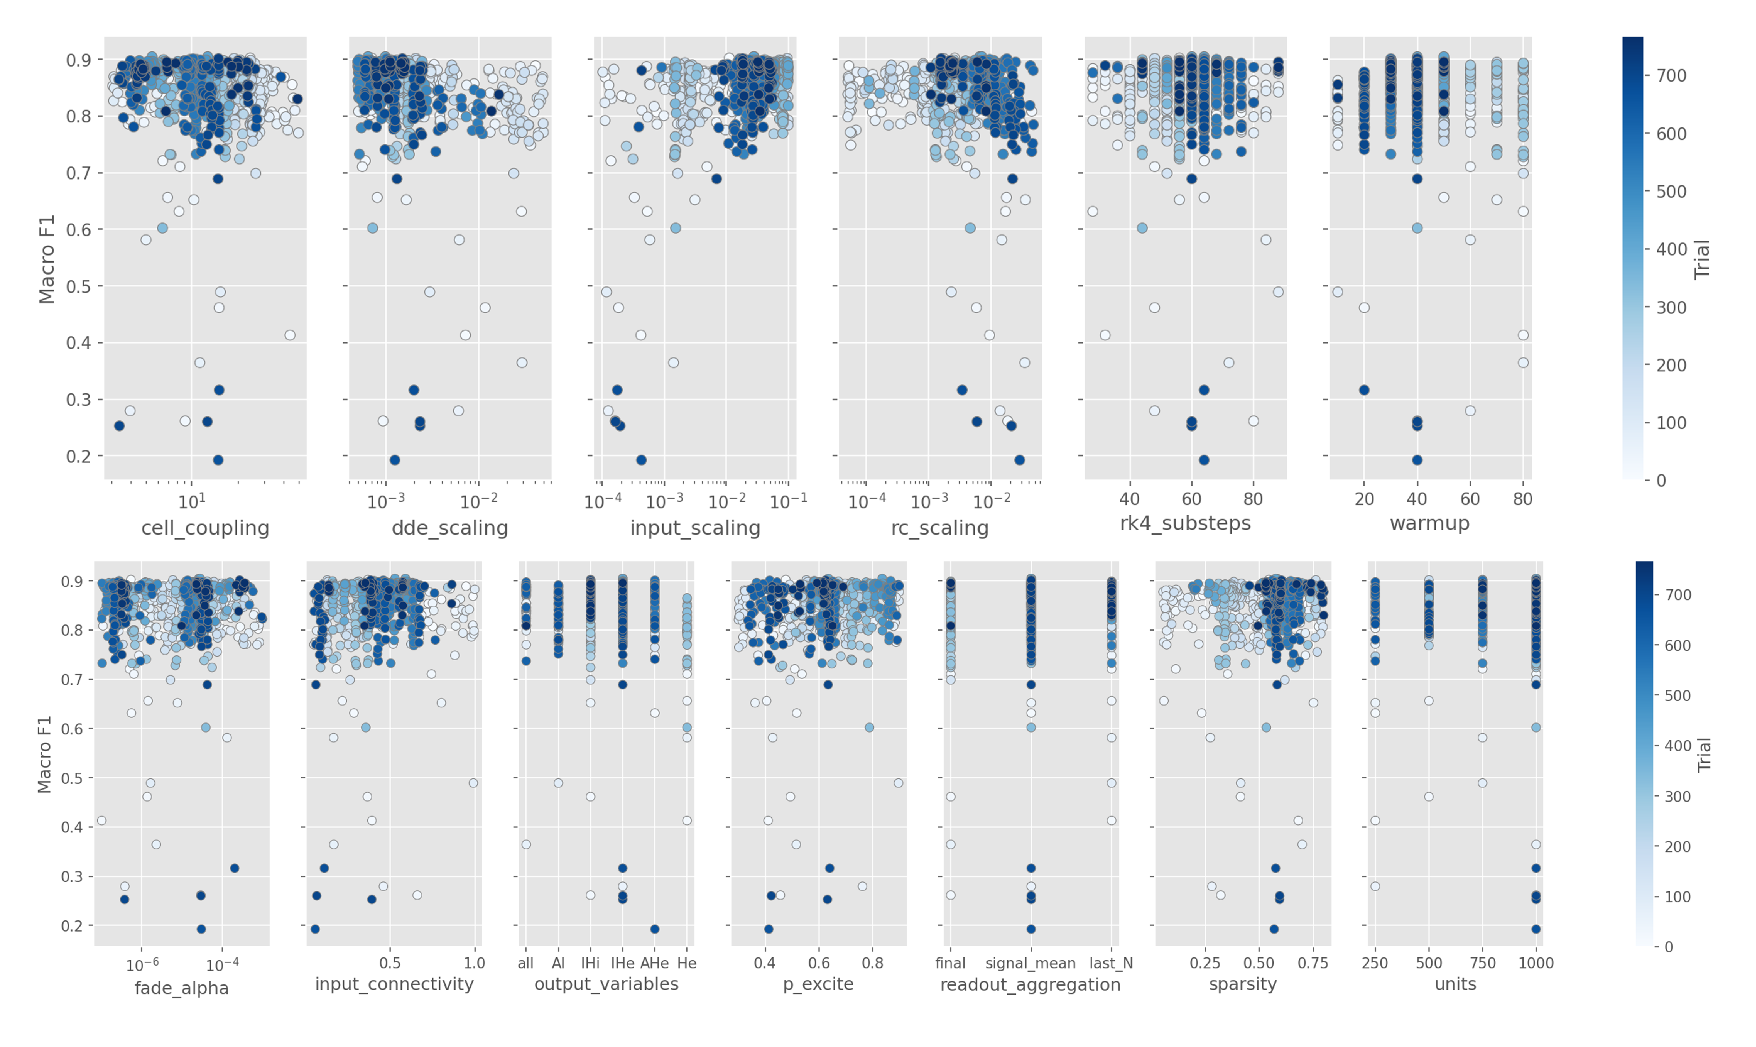
\includegraphics[width=\textwidth]{figures/article/P2-distance-slice.pdf}
    \caption{Optuna slice plot for the Phase~2 joint optimization (P2-distance, distance-based topology, 750 TPE trials). Each panel shows per-trial macro F1-score as a function of one hyperparameter, revealing the marginal sensitivity landscape across 12 jointly optimized parameters.}\label{fig:P2-distance-slice}
\end{figure}

\subsection{Ablation Analysis}
\label{sec:ablation}

Three targeted ablations on the balanced five-class pipeline support the mechanistic claims of the model. Removing recurrent coupling reduced macro F1 from $0.890$ to $0.813$ ($-8.7\%$), removing the transcriptional delay reduced it to $0.809$ ($-9.1\%$), and scrambling the temporal order of each ECG segment collapsed performance to $0.206$, near random. These controls indicate that classification depends on both inter-node coupling and delayed feedback, and that the reservoir is exploiting genuine temporal structure rather than static amplitude statistics alone. Per-fold values and experimental details are reported in Table~S19.


\section{Discussion}
This study demonstrates that reservoirs composed of quorum-sensing genetic oscillators, modeled using experimentally validated kinetic parameters,\cite{Danino2010} can perform competitively on biomedical signal classification tasks. The oscillator reservoir performs strongly on balanced five-class arrhythmia classification and remains competitive under both class imbalance and binary detection, placing it within the performance range of conventional machine learning approaches on the same benchmark.\cite{Kachuee2018} A separately optimized leaky ESN baseline reached $F_1 = 0.878 \pm 0.014$ on the same balanced five-class protocol, so the biological reservoir's advantage is modest but reproducible rather than qualitative; the ESN comparator is a credible, moderately tuned baseline. Crucially, these results are obtained entirely through fixed biological dynamics and a non-parametric readout, without the trainable representational capacity of deep neural networks, highlighting the intrinsic computational utility of coupled gene regulatory dynamics.

Compared to prior molecular reservoir computing approaches, which are implemented in cell-free DNA reaction networks,\cite{Goudarzi2013,Liu2022} the present architecture operates at the gene regulatory level, incorporating transcriptional and translational delays, enzymatic degradation, and diffusive intercellular coupling. These features are absent from the earlier DNA-based reservoirs and arise naturally in living gene circuits~\cite{Goudarzi2013,Liu2022,Danino2010}, positioning quorum-sensing oscillators closer to in vivo implementation. Ahavi et al.~\cite{Ahavi2024} recently demonstrated reservoir computing with living bacterial populations experimentally; the in silico framework presented here complements such efforts by enabling systematic hyperparameter optimization and design-space exploration before committing to costly experimental builds.

Several features of the oscillator reservoir architecture are noteworthy for synthetic biology, and the systematic hyperparameter search yields quantitative design specifications that can guide future wet-lab implementations. The distance-based topology, calibrated to a biologically motivated local length scale informed by Y\'a\~nez et al.,\cite{Yanez2020} outperformed a random Gaussian connectivity baseline ($F_1 = 0.890$ vs.\ $0.881$), indicating that biologically motivated spatial coupling provides a useful inductive bias that stabilizes generalization across data partitions. The reservoir-dynamics visualization in Figure~\ref{fig:reservoir-drive-topology-heatmap} supports this interpretation: strong ECG deflections briefly dominate the net drive, after which locally coupled oscillators relax along distinct trajectories rather than collapsing immediately to the same state, producing the history-dependent state dispersion required for reservoir computing. Reservoir size was a key performance factor, with performance improving up to roughly $N = 250$--$300$ before entering a broad plateau under fixed coupling parameters (Figure~S2), though joint optimization recovered additional benefit at $N = 1000$ by co-adapting coupling and scaling parameters. This plateau suggests a practical target for experimental translation: an array of approximately $250$--$300$ oscillator-bearing microcolonies could capture most of the computational benefit, a scale that appears compatible with previously demonstrated bacterial biopixel arrays.\cite{Prindle2011} Similarly, the optimized coupling-to-input scaling ratio and preferred interaction range (approximately 8 mean nearest-neighbour spacings) provide experimentally testable constraints on trap spacing and inducer delivery rates. Light data augmentation improved generalization, whereas excessive injected noise disrupted the oscillatory dynamics, echoing the sensitivity of living gene circuits to expression noise.\cite{Kaern2005}

The reservoir also benefits substantially from increased training data: performance increased monotonically from $F_1 = 0.882$ to $0.920$ as the majority class was scaled from $1\times$ to $5\times$, and the binary task improved from $F_1 = 0.933$ to $0.961$ when expanded from $4{,}015$ to $37{,}714$ balanced instances. Reservoir computing is often motivated by its fixed dynamics and simple readout,\cite{Konkoli2018} yet these results show that additional data still refines the learned decision boundaries. In this setting, more labeled beats appear to better constrain the geometry of the downstream reservoir-state manifold, allowing the fixed biological dynamics to be partitioned more cleanly by a simple readout without changing the underlying oscillator model. This suggests that for applications where larger datasets are available, genetic oscillator reservoirs can continue to improve without architectural modifications.

\subsection{Computational Cost}
A key limitation is the computational cost of simulating delay differential equations for large oscillator networks. At $N = 1000$, dedicated profiling gave a per-instance simulation cost of approximately \SI{72}{\milli\second}, corresponding to end-to-end five-fold runtimes of roughly 5 minutes for the balanced task, 22 minutes for the unbalanced task, and 52 minutes for the binary task on a 128-core server using five parallel folds. The matched ESN baseline completed the balanced five-fold run in under 2 minutes on the same host. More than 95\% of wall-clock time is spent in DDE integration, so runtime scales mainly with the number of evaluated instances rather than with readout fitting (Table~S2). This computational overhead matters for large-scale in silico benchmarking, but it does not undermine the central motivation of the work: in a physical implementation, the nonlinear dynamics would be instantiated directly rather than numerically integrated.

\subsection{Limitations}
Several limitations should be considered when interpreting these results. First, all experiments used a single benchmark dataset, and the balanced five-class setting remains relatively small ($4{,}015$ instances). Although MIT-BIH is a standard reference,\cite{Moody2001} generalization to other temporal tasks and larger datasets remains to be demonstrated. In addition, the Kachuee preprocessing uses beat-wise rather than patient-wise splitting, so cross-validation folds may contain beats from the same patient. That choice matches the source release and is difficult to avoid for balanced five-class evaluation because the minority classes are concentrated in very few records, but it likely yields more optimistic performance than a strict patient-wise protocol.\cite{Kachuee2018,deChazal2004}

Second, the reported five-fold scores are post-selection estimates. Phases~1--2 used a single fold as a proxy during optimization, and we did not run fully nested cross-validation because the multi-phase search was already computationally expensive. The fold-to-fold standard deviations therefore capture sampling variability of the selected model, not the full uncertainty introduced by model selection.

Third, the current implementation is a proof-of-concept simulation rather than a near-term real-time device model. The DDE solver runs in dimensionless computational time, whereas the Danino oscillator operates on roughly hour-scale periods in vivo,\cite{Danino2010} so a physical implementation would require recorded inputs to be replayed over biological timescales. The system is therefore better interpreted as an offline biological coprocessor than as a real-time monitor.

Finally, the biological model remains idealized. It omits growth, division, metabolic burden, and flow-induced anisotropy, and it treats some device-calibrated density terms as fixed rather than dynamic. We partially addressed biological realism through a dedicated heterogeneity analysis: performance remained close to baseline across low-to-moderate node-to-node kinetic variability, suggesting that the reservoir is reasonably robust to experimentally plausible cell-to-cell variation,\cite{Elowitz2002,Taniguchi2010,Raj2008,Danino2010} but fuller in vivo validation is still required.

\subsection{Software and Reproducibility}
The modular open-source software platform developed for this study\cite{JamesGitHub2024} decouples oscillator models, reservoir topology, and readout algorithms, enabling researchers to substitute components, benchmark alternative designs, and test hypotheses without modifying the simulation core. The codebase includes comprehensive unit tests to ensure correctness, classification pipeline profiling, per-fold and per-class metric analysis, and detailed analysis and visualisation tools for cross-validation diagnostics. All experiments are fully reproducible with fixed random seeds and pinned dependency versions. The framework requires only a standard Python environment with no specialized hardware, lowering the barrier to adoption for synthetic biology groups exploring computational gene circuit applications.

\subsection{Potential Applications}
The most immediate contribution of this work is methodological rather than application-specific: it provides a structured software framework for simulating, visualizing, benchmarking, and stress-testing biologically grounded reservoir architectures before committing to experimental builds. In that role, the ECG task functions as a demanding temporal benchmark rather than as a near-term clinical product, allowing the reservoir to be compared against conventional baselines under controlled conditions.
Even so, the broader application space remains relevant: oscillator-based temporal classifiers are plausible in biosensing and monitoring settings where noisy sequential signals must be interpreted under tight power or integration constraints, including gut-resident diagnostics, physiological forecasting, livestock disease surveillance, and environmental sensing.~\cite{Chancharoenthana2023,Guerra2023,Wang2022,Negahdary2023}

The longer-term opportunity is hybrid wet-lab implementation. A plausible realization would use trapped microcolonies as reservoir nodes and combine microfluidic signal delivery or electrogenetic actuation with optical measurement of a small set of reporter channels for downstream classification.~\cite{Danino2010,Prindle2011,Tschirhart2017,Rackus2015} Prior demonstrations of multicellular NOR-gate circuits and layered intracellular logic indicate that at least some downstream decision logic could, in principle, also be implemented genetically rather than digitally.~\cite{Tamsir2011,Moon2012} In this setting, the present study offers experimentally useful design constraints on reservoir size, coupling locality, and observable state variables, while the software platform provides a practical bridge between in silico exploration and future biological prototypes. Previously demonstrated bacterial biopixel arrays and oscillator-based biosensing systems make that translational direction concrete rather than purely speculative.~\cite{Prindle2011} Such systems may ultimately support biosensing or low-power hybrid bioelectronic classifiers, but the main significance here is demonstrating that experimentally grounded genetic dynamics can encode discriminative temporal structure in a form usable for machine-learning-style classification.

\section{Methods}

\subsection{Simulating Gene Expression in Quorum-Coupled Bio-Pixels}
The reservoir consists of an array of genetic “bio-pixels” modeled as quorum-sensing transcriptional oscillators derived from the synchronized genetic clock reported by Danino et al.~\cite{Danino2010}. The dynamical equations are identical to those reported in that work, except for discretization and the addition of external input forcing. Here we describe the single-node dynamical model; integration into the reservoir architecture is detailed in a subsequent section.

Quorum sensing in Gram-negative bacteria is mediated by diffusible \textit{N}-acyl homoserine lactones (AHLs), synthesized by LuxI-family enzymes and detected by LuxR-type transcriptional regulators to coordinate population-level gene expression.\cite{Fuqua2002} In the Danino oscillator, LuxI produces AHL, which binds LuxR and activates the \textit{PluxI} promoter, driving expression of both \textit{luxI} and the AHL lactonase \textit{aiiA}. AiiA hydrolyzes AHL, attenuating quorum signaling.\cite{Dong2000} This delayed activator–inhibitor architecture forms a positive–negative feedback loop capable of sustained oscillatory dynamics and synchronization.\cite{Danino2010} LuxR was assumed to be constitutively expressed and was not modeled explicitly, consistent with the reduced-order formulation of Danino et al.

For each bio-pixel $j$, the state variables are intracellular LuxI ($I^{(j)}$), intracellular AiiA ($A^{(j)}$), intracellular AHL ($H_i^{(j)}$), and a local extracellular AHL variable ($H_e^{(j)}$). The extracellular variable represents a per-cell microenvironment; no shared extracellular pool was modeled, coupling is handled at the reservoir level. Each node should therefore be interpreted as a mean-field surrogate for a small trapped microcolony with population-averaged dynamics, rather than as a literal single cell.

Promoter activation is described by a delayed Hill-type response,
\begin{equation}
    P(t) =
    \frac{\delta + \alpha H_i(t-\tau)^2}
    {1 + k_1 H_i(t-\tau)^2},
\end{equation}
where $\tau$ represents effective transcriptional and translational latency.

The bio-pixel dynamics are given by
\begin{align}
    \frac{dA}{dt} &=
    C_A \left[1 - \left(\frac{\rho}{\rho_0}\right)^4 \right]
    P(t)
    - \frac{\gamma_A A}{1 + f (A + I)}, \\
    \frac{dI}{dt} &=
    C_I \left[1 - \left(\frac{\rho}{\rho_0}\right)^4 \right]
    P(t)
    - \frac{\gamma_I I}{1 + f (A + I)}, \\
    \frac{dH_i}{dt} &=
    b \frac{I}{1 + k I}
    - \frac{\gamma_H A H_i}{1 + g A}
    + D (H_e + x_t - H_i), \\
    \frac{dH_e}{dt} &=
    -\frac{\rho}{1 - \rho} D (H_e - H_i)
    - \mu H_e,
\end{align}
where $x_t$ denotes an externally applied input signal at time $t$, modeled as an additive perturbation to the effective extracellular drive term entering the diffusion flux into $H_i$. The density parameters $\rho$ and $\rho_0$ are treated as fixed constants inherited from Danino et al., so the associated growth-modulation factor is not itself dynamically updated during simulation.

All biological rate constants, parameter values, and units were adopted directly from the experimentally validated model of Danino et al.~\cite{Danino2010} and are listed in Table~S1. No intrinsic kinetic parameters were tuned for classification experiments.

The DDEs evolve in continuous time; for simulation, time was discretized with step size $\Delta t$ defining one timestep. $\Delta t$ was set equal to the interval between consecutive input measurements (see Dataset Preprocessing section for sampling frequency), so that one timestep corresponds to one input sample. The delay was fixed at $\tau = 10$ discrete timesteps for all simulations and was not varied across experiments. Delayed terms were implemented using a rotating history buffer storing the previous 10 states of $H_i$ per node. The delay differential equations were integrated using a Method-of-Steps fourth-order Runge–Kutta (RK4) scheme. Within each external timestep, the delayed value $H_i(t-\tau)$ was evaluated once by linear interpolation of the history buffer and held constant across the four RK4 stages (frozen-delay formulation). Each external timestep was resolved using 64 RK4 substeps unless otherwise specified. The observed first-order global convergence arises because the frozen-delay formulation evaluates the delayed term once per external timestep, thereby limiting the overall scheme to $\mathcal{O}(h^1)$ accuracy irrespective of the fourth-order ODE integrator. The frozen-delay approximation constrains global convergence to $\mathcal{O}(h^1)$; however, the fourth-order RK4 integrator reduces local truncation error in the non-delayed terms evaluated within each timestep. Convergence was verified against a scalar DDE with closed-form solution across a 64-fold refinement range (Figure~S1), yielding fitted slopes of 1.00–1.01. The production solver was further validated on the biological model by comparing 24, 48, and 64 substeps against a 96-substep reference trajectory (Figure~S2). At 64 substeps, the accumulated relative error in $H_i$ over 50 timesteps was well below $10^{-4}$, substantially smaller than estimated biological parameter uncertainty ($\sim 10\%$).\cite{Gutenkunst2007} All state variables remained non-negative.

Initial conditions were sampled independently for each bio-pixel from log-normal distributions with log-space parameters $(\mu, \sigma)$ representing low basal expression: $I$ and $A$ $(\mu=-2.0,\sigma=0.5)$, $H_i$ $(\mu=-4.0,\sigma=0.3)$, and $H_e$ $(\mu=-3.0,\sigma=0.3)$. Randomized low-expression initialization is standard practice in modeling synthetic gene oscillators and does not affect long-term limit-cycle behavior.\cite{Elowitz2000, Danino2010} To eliminate transient dependence on initialization, simulations employed a zero-input warmup phase ($x_t = 0$). Stability was assessed by visual inspection of representative trajectories, (see ``Baseline'' from Figure~\ref{fig:biopixel-reservoir-oscillations}b) to confirm steady limit-cycle behavior and invariance of downstream classification accuracy. Warmup durations between 30--120 timesteps satisfied these criteria; unless otherwise stated, 50 timesteps were used.

\begin{figure}
    \centering
    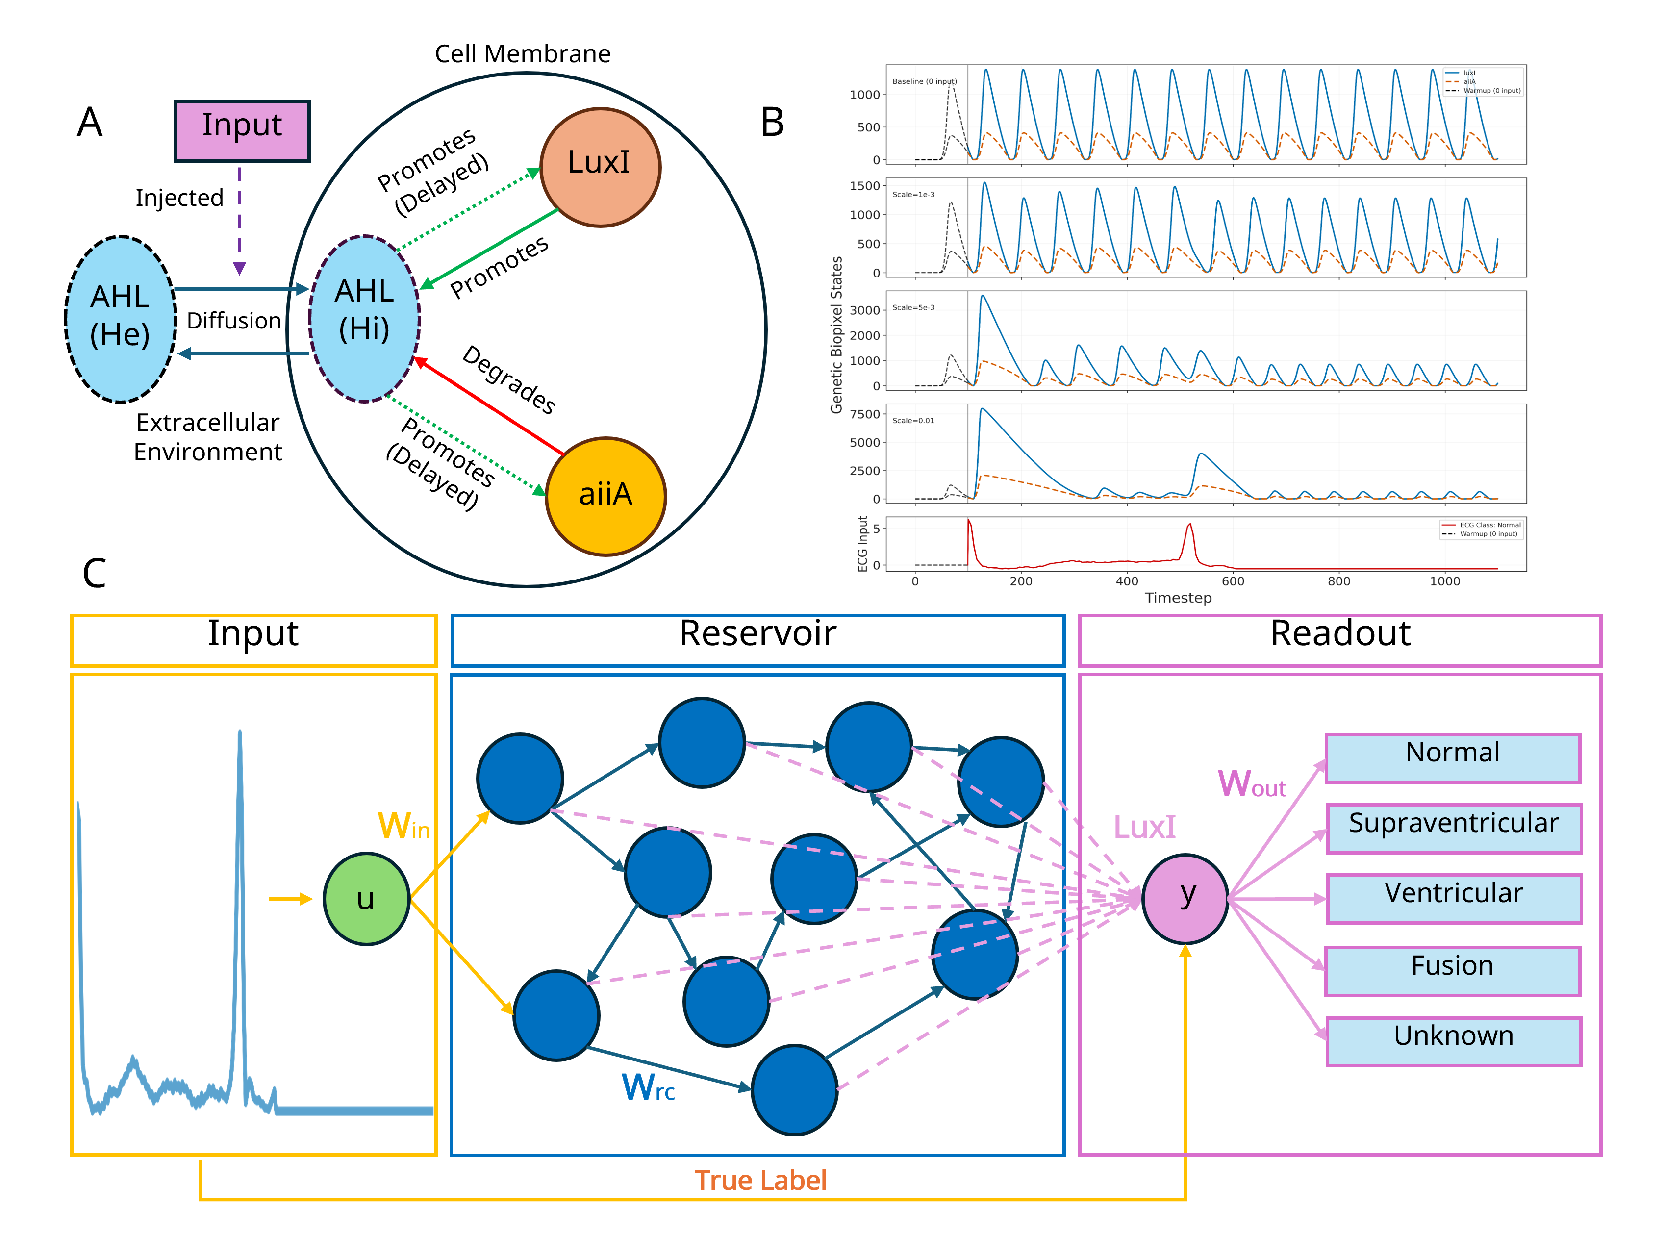
\includegraphics[width=0.9\linewidth]{figures/article/biopixel-reservoir-model-3-subfigures.pdf}
    \caption{Overview of the genetic bio-pixel model, its effective input scales, and our reservoir computing architecture. (a) Schematic of a quorum-sensing genetic oscillator adapted from Danino et al., comprising the autoinducer synthase \textit{luxI}, the AHL lactonase \textit{aiiA}, intracellular AHL ($H_i$), and extracellular AHL ($H_e$). AHL freely diffuses across the membrane, coupling intracellular and extracellular pools. Intracellular AHL activates transcription of \textit{luxI} and \textit{aiiA} through delayed positive feedback (modeled via Hill-type promoter activation), while AiiA degrades AHL, forming a negative feedback loop that generates oscillatory dynamics. External inputs are modeled as perturbations to the effective extracellular drive term $(H_e + x_t)$ entering the diffusion flux into $H_i$. (b) Representative time-series of a single bio-pixel under varying input amplitudes, using a rescaled ECG waveform applied through this effective extracellular drive term. Increasing input strength alters oscillation amplitude, phase, and transient response, demonstrating nonlinear dynamical behavior. A warmup period precedes stimulus-driven dynamics. (c) Reservoir computing architecture in which spatially distributed bio-pixels communicate through diffusive AHL signaling with distance-dependent coupling. A univariate ECG signal is injected per timestep, and the reservoir state is defined by the intracellular LuxI and extracellular AHL concentrations across nodes. The trajectory-averaged state vector is supplied to a readout classifier for heartbeat classification.}\label{fig:biopixel-reservoir-oscillations}
\end{figure}

\subsection{Reservoir Architecture and Topology}
The reservoir consists of $N$ genetically inspired nonlinear oscillator units arranged in a two-dimensional spatial domain. Each node is assigned coordinates uniformly sampled in the unit square $[0,1]^2$, representing spatially distributed microbial populations. Recurrent connectivity is defined through a distance-dependent interaction kernel:

\begin{equation}
W_{ij} = \exp\!\left(-\left(\frac{D_{ij}}{\ell}\right)^2\right),
\end{equation}

where $D_{ij}$ denotes the Euclidean distance between nodes $i$ and $j$, and $\ell$ is a characteristic interaction length scale.

To provide a biologically interpretable parameterization, the interaction range was specified in units of mean nearest-neighbor distance (``cell diameters''). Given an interaction range $R$ and fade level $\alpha = 0.01$, the corresponding length scale was computed as:

\begin{equation}
\ell = \frac{R}{\sqrt{-\ln \alpha}}.
\end{equation}

Unless otherwise noted, we used $R \approx 8.2$, chosen as a biologically motivated local length scale rather than as a direct measurement of AHL diffusion. This value matches the order of the $r_0 = 8.23 \pm 1.69$ cell radial length scale reported for dense bacterial colonies by Y\'a\~nez et al.~\cite{Yanez2020}.

Connections beyond radius $R$ were optionally removed via geometric cutoff, enforcing locality consistent with diffusive quorum sensing interactions. Recurrent weight signs were determined by a Bernoulli random variable with excitatory probability $p_{\mathrm{excite}}$; each non-zero weight was multiplied by $+1$ (excitatory) or $-1$ (inhibitory) accordingly. Pure diffusive coupling ($p_{\mathrm{excite}} = 1$) did not significantly differ from mixed signed connectivity during Phase~1 exploration (Figure~S8); however, the joint Phase~2 optimization converged to $p_{\mathrm{excite}} \approx 0.84$, yielding a predominantly excitatory but partially inhibitory coupling matrix. Signed connectivity was therefore used for all reported classification experiments. We note that passive AHL diffusion is inherently excitatory: a single quorum-sensing molecule cannot activate one neighbour and inhibit another without additional genetic circuitry~\cite{Fuqua2002,Danino2010}. Realising inhibitory recurrent connections in vivo would require a multi-strain consortium in which a subpopulation carries an inverted circuit---for example, one where AHL activates a fast-acting repressor such as TetR that suppresses the target promoter. Because Phase~1 showed negligible performance difference between $p_{\mathrm{excite}} = 1$ and mixed-sign coupling, a simpler purely excitatory architecture ($p_{\mathrm{excite}} = 1$) may therefore be preferable for initial experimental builds. Following construction, the recurrent matrix was normalized to unit spectral radius ($\rho(W) = 1$).

During simulation, the matrix was scaled by a recurrent gain parameter $\alpha_r$, such that the effective linear spectral radius was $\alpha_r$. For the values used here ($\alpha_r \sim 10^{-2}$), the reservoir operates well below the classical echo-state regime in which recurrent dynamics are self-sustaining rather than input-driven~\cite{Jaeger2001,Nakajima2020}. Instead, nonlinear dynamics arise intrinsically from the underlying genetic oscillator model rather than from linear recurrence. Where specified, additional random sparsification (density parameter $s$) was applied. Sparse matrices were stored in CSR format to accelerate matrix--vector products for large $N$. Each ECG segment was represented as a univariate time series $u(t)$. Input weights were drawn from a Bernoulli distribution over $\{-1, +1\}$ with probability $p = 0.5$, with partial connectivity (input\_connectivity $\approx 0.53$) such that approximately half the reservoir nodes received direct input at each timestep. Physically, a global inducer pulse can only increase local concentration; realising negative input weights (where an increase in signal amplitude reduces the effective drive) would require an inhibitory bio-pixel variant in which the inducer drives a repressor (e.g., LacI) that attenuates the oscillator's promoter, thereby inverting the input sign genetically.

The external drive applied to node $i$ at time $t$ was defined as:

\begin{equation}
x_i(t) = \lambda \alpha_u w^{\mathrm{in}}_i u(t),
\end{equation}

where $\alpha_u$ is the input scaling parameter and $\lambda$ is the DDE input coefficient controlling the strength of perturbation to the oscillator dynamics. No per-timestep normalization of the input drive was applied. Earlier experiments using instantaneous variance normalization did not measurably affect classification performance and were therefore removed to preserve biological interpretability.

Single-node amplitude sweep experiments (Figure~\ref{fig:biopixel-reservoir-oscillations}b) demonstrated sustained oscillatory dynamics for perturbation magnitudes approximately satisfying $|x(t)| \lesssim 5 \times 10^{-3}$. All reported experiments used combinations of $\lambda$ and $\alpha_u$ such that $|x_i(t)|$ remained within this empirically characterized oscillatory regime. This ensured that reservoir dynamics reflected modulated oscillatory behavior rather than damped or unstable trajectories.

Reservoir dynamics were simulated using a fourth-order Runge--Kutta (RK4) integrator with fixed timestep $\Delta t$. For each external input timestep, multiple RK4 substeps were computed. Two distinct aggregation mechanisms were employed. First, \textit{RK4 state aggregation} ($K_{\mathrm{RK4}}$): within each external timestep, the states from the final $K_{\mathrm{RK4}}$ RK4 substeps were averaged to reduce high-frequency numerical fluctuations. Second, \textit{readout state aggregation} ($K_{\mathrm{readout}}$): for each input segment, a subset of reservoir states was supplied to the readout. We evaluated aggregation over the first $K_{\mathrm{readout}}$ timesteps, the last $K_{\mathrm{readout}}$ timesteps, or the full trajectory mean, allowing the readout to exploit transient or steady-state dynamics. Phase~2 optimization selected the full trajectory mean, yielding a single time-averaged state vector per segment. Two of the four node state variables---intracellular LuxI ($I$) and extracellular AHL ($H_e$)---were selected as observed outputs, giving a $2N$-dimensional feature vector for $N$ reservoir nodes. These two aggregation hyperparameters were optimized independently. Reservoir state was reset between ECG segments to prevent inter-instance information leakage. Unlike streaming reservoir deployments where state persists across inputs, each ECG segment was treated as an independent labeled instance. The aggregated reservoir state vector for each instance was supplied to a trainable readout layer; only readout weights were trained, and all reservoir parameters remained fixed after initialization. The readout algorithm was selected via hyperparameter optimization (see below): $k$-nearest neighbors was used for five-class tasks, and random forest for binary classification.
 
\begin{figure}
    \centering
    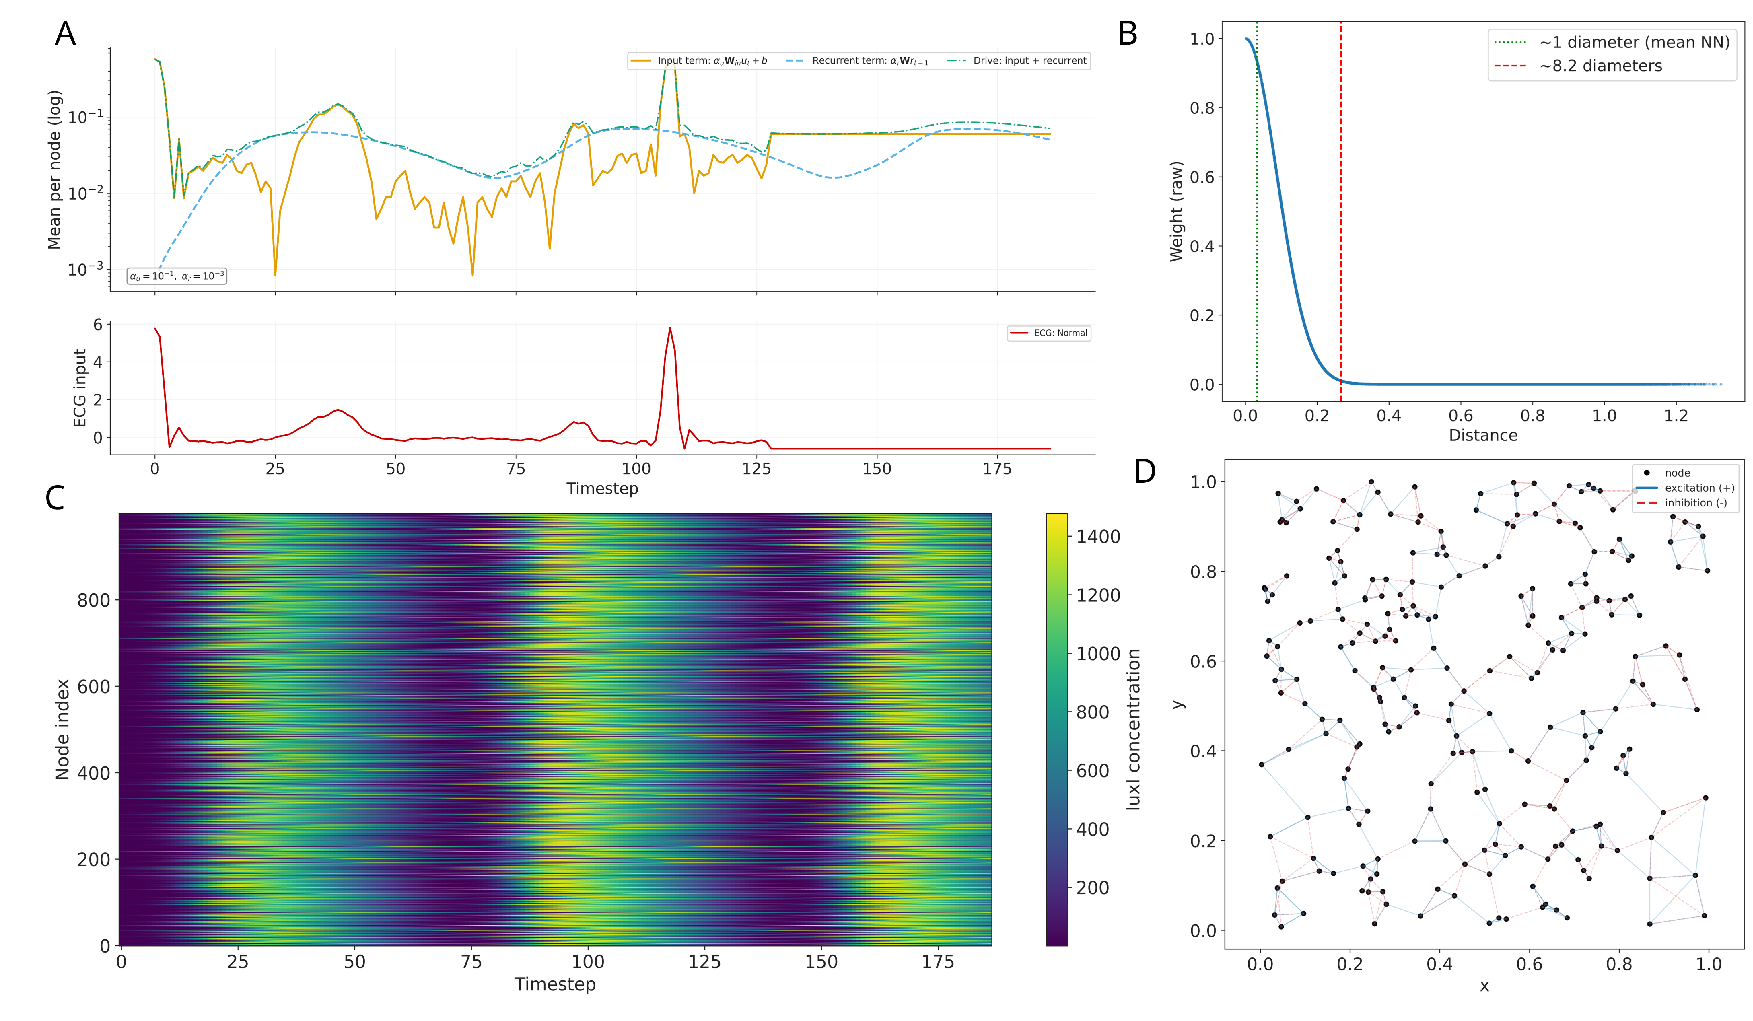
\includegraphics[width=0.84\linewidth,height=0.42\textheight,keepaspectratio]{figures/article/reservoir_drive_topology_heatmap.pdf}
    \caption{Characterization of reservoir dynamics and spatial topology using effective parameters chosen for visualization rather than for the headline classification runs. $N=1000$ nodes were used for panels (a) and (c) with input and recurrent scaling coefficients $\alpha_u=10^{-2}$ and $\alpha_r=10^{-4}$, respectively; panels (b) and (d) use $N=250$ nodes. These settings were selected because they make the dynamical decomposition visually legible; the optimized classification parameters produce the same qualitative pattern of input-dominated transients followed by locally coupled relaxation, but with smaller absolute magnitudes and denser overlap between traces. (a) Mean absolute magnitude of the input contribution ($\alpha_u \mathbf{W}_{\mathrm{in}} u_t + b$), recurrent contribution ($\alpha_r \mathbf{W} r_{t-1}$), and their sum (net drive), averaged across reservoir nodes at each timestep (log scale). The lower subplot shows the corresponding ECG waveform after per-sequence standardization and prior to input scaling. Input-driven dynamics dominate during high-amplitude ECG phases, whereas recurrent interactions sustain activity during quiescent intervals, consistent with a short fading-memory mechanism in which ECG-driven perturbations decay over several subsequent steps rather than instantaneously. (b) Distance-dependent coupling kernel for inter-node communication. Interaction strength decays exponentially with distance (measured in cell-diameter units estimated from mean nearest-neighbour spacing) and is truncated at an interaction radius of approximately 8.2 cell diameters, chosen to match the order of the $r_0 = 8.23 \pm 1.69$ cell radial length scale reported for dense bacterial colonies by Y\'a\~nez et al.~\cite{Yanez2020}. (c) Temporal evolution of intracellular LuxI concentration across all nodes for a single ECG instance. The intrinsic oscillation period is approximately 60 timesteps. Progressive dispersion of node trajectories illustrates expansion of the one-dimensional input into a high-dimensional dynamical state through coupled phase and amplitude modulation across the oscillator population. (d) Spatial realization of the reservoir as a two-dimensional colony. Nodes are randomly positioned; signed edges denote effective excitatory and inhibitory interactions within the local interaction radius, connections are highly localised due to the short interaction range defined by the distance kernel described in panel~(b), matching the biologically plausible local coupling regime used throughout the study.}\label{fig:reservoir-drive-topology-heatmap}
\end{figure}


\subsection{Dataset Processing}
We used the MIT-BIH Arrhythmia Database~\cite{Moody2001} in the pre-segmented form released by Kachuee et al.~\cite{Kachuee2018}. In the CSV release used here, the working dataset contains 109,446 single-heartbeat ECG segments sampled at 125\,Hz with 187 samples per beat ($\approx$1.5\,s duration). Following the five-class heartbeat grouping used by Kachuee et al. in accordance with the AAMI EC57 standard~\cite{AAMI1998}, beats were labeled as Normal (N), Supraventricular ectopic (S), Ventricular ectopic (V), Fusion (F), and Unknown (Q). Class-averaged waveforms and intra-class variability are shown in Figure~\ref{fig:dataset-figure}a. For the balanced five-class task, each class was subsampled to the smallest class size (Fusion, 803 samples), yielding 803 samples per class (4\,015 total). This pool was evaluated using stratified five-fold cross-validation, with each fold producing approximately 643 training and 160 test samples per class. For the unbalanced task, a balanced reserve set of 160 beats per class (800 total) was held out before applying the per-class cap; the effective cross-validation pool size is therefore the capped pool plus this 800-instance reserve (see Table~\ref{tab:imbalance-scaling}). Labels were one-hot encoded for multi-class classification.

The raw ECG segments in the Kachuee CSV files are amplitude-scaled to $[0,1]$ at source~\cite{Kachuee2018}. We applied per-sequence z-score normalization on top of this representation, replacing the source scaling for all downstream processing (Figure~\ref{fig:dataset-figure}c). Per-sequence normalization yielded superior classification performance over global z-score and was therefore used in all reported experiments. Because normalization statistics were computed independently for each individual sequence, no information from the test set influenced training, preventing data leakage. To improve generalization, additive Gaussian noise augmentation was applied: for approximately 29\% of each class's training samples, a noisy copy was generated by perturbing the original waveform with zero-mean Gaussian noise scaled to 30\% of the per-sequence standard deviation. Augmented samples were appended to the training set to increase its size, as illustrated in Figure~\ref{fig:dataset-figure}b. Augmented samples were included only in the training set. In addition to five-class classification, we evaluated a binary task in which all non-normal classes were merged into a single arrhythmia category, ensuring to balance classes to the smallest class size again.

\begin{figure}
    \centering
    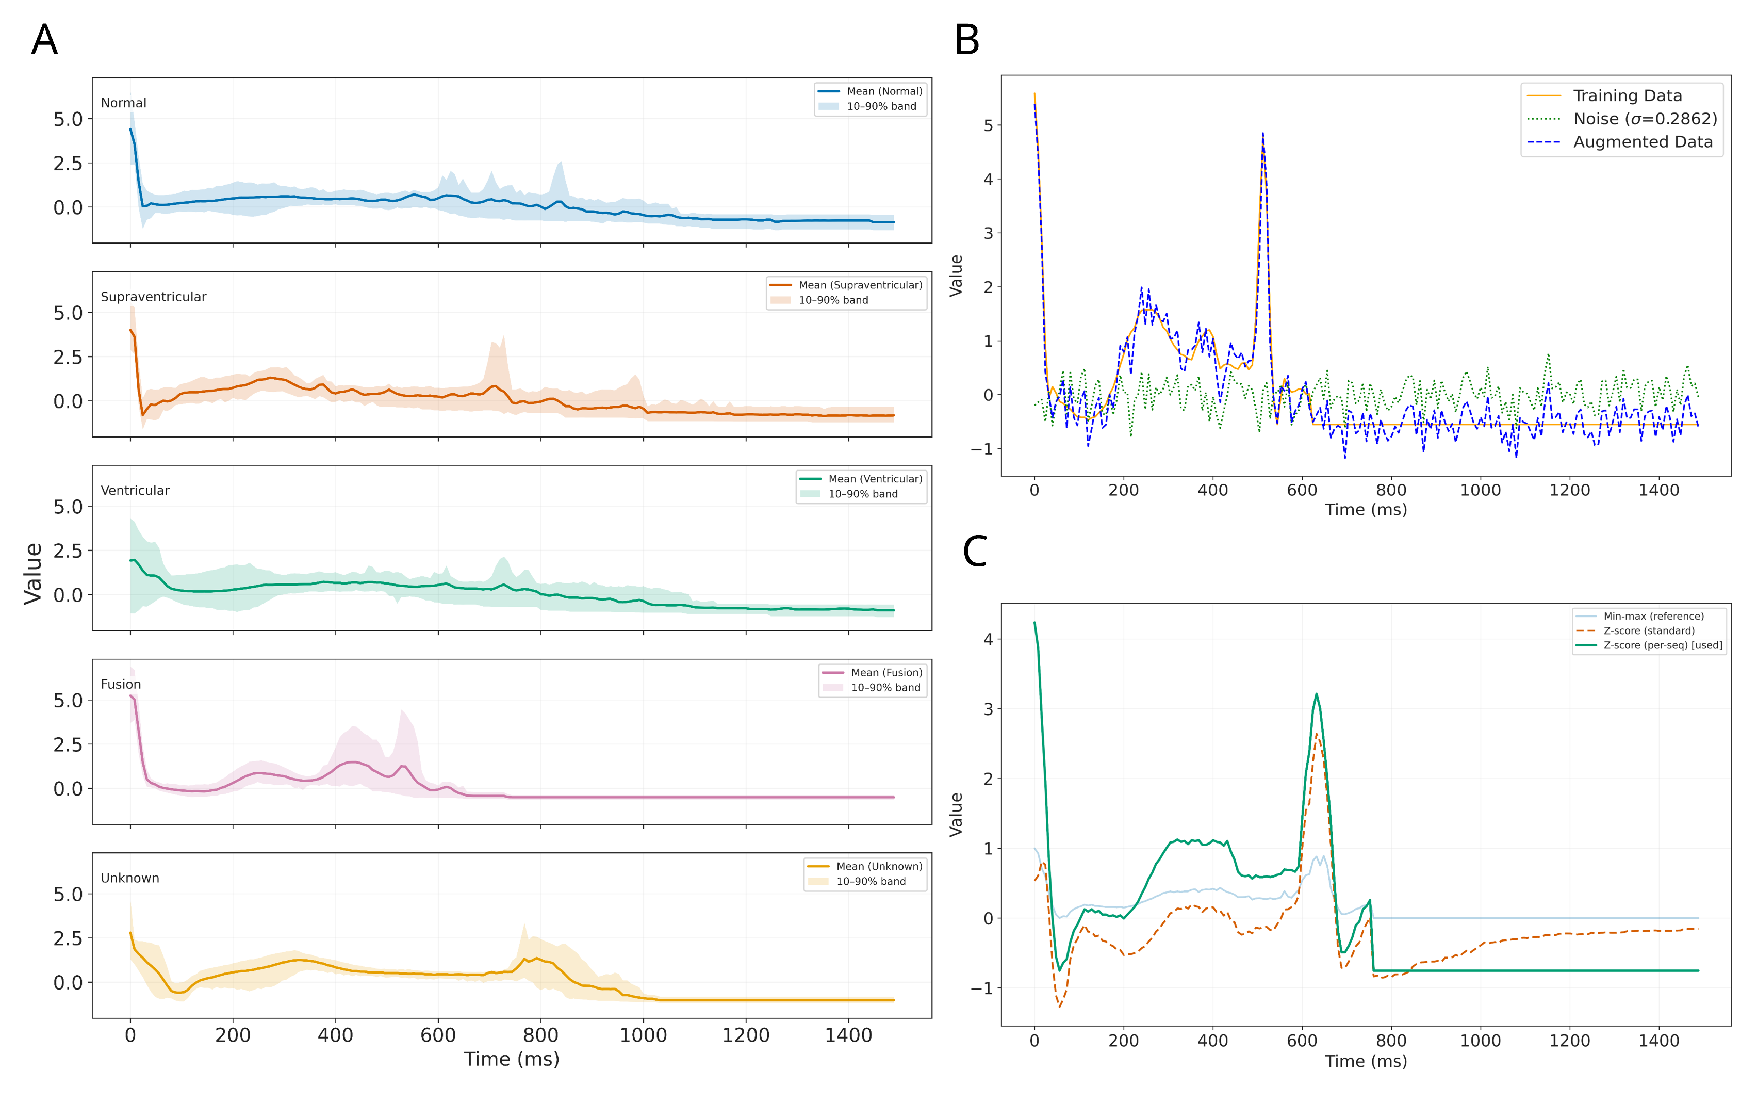
\includegraphics[width=1\linewidth]{figures/article/samples_noise_scalers-subfigures.pdf}
    \caption{ECG dataset characterization, augmentation, and preprocessing strategies. (a) Class-averaged ECG waveforms for each heartbeat category (Normal, Supraventricular, Ventricular, Fusion, and Unknown). Solid lines denote the mean waveform across samples within each class, and shaded regions indicate the 10--90\% percentile range at each timepoint, illustrating intra-class variability. (b) Example of additive Gaussian noise augmentation applied to a single ECG instance. The original waveform (training data) is perturbed by zero-mean Gaussian noise scaled to a fraction of the sequence standard deviation, generating augmented samples while preserving overall waveform morphology. (c) Comparison of normalization strategies applied to an ECG sequence. The reference signal is shown after min–max scaling to $[0,1]$. Standard global z-score normalization and per-sequence (sample-wise) z-score normalization are overlaid for comparison. Per-sequence z-score normalization was used for classification experiments because it preserves beat morphology while removing across-beat amplitude bias, which is more relevant to this task than absolute signal scale.}\label{fig:dataset-figure}
\end{figure}

\subsection{Classification Methodology}
Classification was performed using a reservoir computing framework in which the quorum-sensing oscillator network served as a fixed, untrained dynamical reservoir, and only the readout layer was optimized. Model performance was evaluated using stratified five-fold cross-validation. For each fold, the dataset was randomly shuffled (fixed seed) and split into training (80\%) and test (20\%) subsets while preserving class proportions. Noise augmentation was applied exclusively to the training set after splitting. All preprocessing procedures were applied independently within each fold. During training, each ECG sequence was sequentially injected into the reservoir as a time-varying input signal. The coupled delay differential equations governing the reservoir were numerically integrated for the duration of the sequence, and the trajectory-mean reservoir state vector (averaged across all timesteps) was recorded as a fixed-dimensional representation of the input. To prevent state carryover between samples, the reservoir state and internal delay buffers were reset to identical initial conditions prior to processing each sequence. The same evaluation pipeline was also applied to a standard leaky ESN comparator implemented in ReservoirPy, so the baseline differed only in reservoir dynamics rather than preprocessing, metric semantics, or readout-selection procedure.

After collecting state vectors for all training samples, the readout layer was fitted using the corresponding ground-truth labels. The reservoir weights remained fixed throughout all experiments. The same procedure was then applied to the test set to obtain state representations, which were passed to the trained readout to generate predictions. Seven readout classifier families were evaluated during Phase~4 hyperparameter optimization (see below), including $k$-nearest neighbors (KNN), random forest, gradient boosting, ridge classifier, logistic regression, SVM, and decision tree. KNN yielded the best five-class performance and random forest the best binary performance; these were used for all reported headline results. For each fold, classification performance was quantified using accuracy, precision, recall, macro F1-score, weighted F1-score, Matthews correlation coefficient (MCC), and Cohen's $\kappa$. Macro F1 is used as the primary optimization and headline reporting metric because it weights classes equally, whereas weighted F1 is retained as a secondary summary for imbalanced settings. Final reported metrics correspond to the mean and standard deviation across the five folds.

\subsection{Hyperparameter Optimization}
Hyperparameter optimization was performed using Optuna~\cite{Akiba2019} with a Tree-structured Parzen Estimator (TPE) sampler, following a four-phase hierarchical strategy for the biological reservoir and a separate comparator track for the ESN baseline. Macro-averaged F1-score on the balanced five-class ECG classification task served as the primary objective metric throughout, with weighted F1 tracked in parallel for imbalanced result interpretation. Studies were distributed across dedicated servers running RHEL~9 (Intel Xeon Gold 6538Y+, 64 physical cores per host), with between 12 and 64 asynchronous parallel workers per host sharing a single SQLite-backed Optuna study database, enabling concurrent trial evaluation without inter-worker coordination overhead.

\textit{Phase~1} comprised eleven independent single-factor sensitivity studies, each isolating one parameter group while all other parameters were held fixed at a shared baseline configuration. To reduce computational cost during the exploratory phase, each trial was evaluated on a single stratified cross-validation fold (4015 instances, 80/20 train/test split). Per-trial wall time ranged from approximately 430 to 1250\,s at $N = 250$ reservoir nodes, with peak memory usage below 600\,MB per worker. Trial budgets ranged from 30 trials using a grid sampler for the categorical scaler selection study, to 288 TPE trials for the signal amplitude scaling study. The parameter groups examined in Phase~1 were: (i)~dataset normalization strategy, (ii)~signal amplitude scaling coefficients, (iii)~DDE numerical integration parameters, (iv)~distance-based topology structural parameters, (v)~random Gaussian topology parameters, (vi)~inter-nodal coupling strength, (vii)~input layer connectivity and observed reservoir state variables, (viii)~readout aggregation strategy, (ix)~data augmentation noise, (x)~reservoir process noise, and (xi)~reservoir size. Baseline parameter values were updated from Phase~1 best-trial results before initiating Phase~2.

\textit{Phase~2} comprised two parallel joint refinement studies (P2-distance: distance-based topology; P2-random: random Gaussian topology), each searching all salient reservoir, DDE integration, topology, input, and readout parameters simultaneously over 750 TPE trials on a single fold. Running both topology variants under an identical trial budget and parameter search space corrected for the confounding present in Phase~1, where the shared baseline parameters had been established under a distance-topology prior. The best Phase~2 configuration was selected as the final model for downstream evaluation.

\textit{Phase~3} evaluated the best Phase~2 configuration (P2-distance, distance-based topology) under two additional task settings using five-fold stratified cross-validation. First, a grid search over the maximum samples per class ($1\times$--$5\times$) characterized performance under increasing class imbalance. Second, a binary classification variant (Normal vs.\ Arrhythmia) was assessed using the same reservoir parameters.

\textit{Phase~4} optimized the readout classifier on frozen reservoir states generated by the Phase~2/3 configurations. Seven classifier families (KNN, gradient boosting, random forest, ridge, logistic regression, SVM, decision tree) were evaluated with classifier-specific hyperparameters searched via TPE, using five-fold cross-validation F1-score as the objective. This phase isolated the contribution of readout algorithm selection from reservoir dynamics. Complete search ranges, best-trial parameter values, and per-study performance summaries are provided in the Supporting Information (Tables~S5--S16; Figures~S5--S16).

In addition to these four BioReservoir phases, we ran a separate ESN comparator track using ReservoirPy. The ESN training study optimized reservoir size, input scaling and connectivity, recurrent connectivity, spectral radius, leak rate, activation, bias, and noise over 256 planned TPE trials on the same balanced single-fold proxy task; the best ESN states were then passed into a separate 548-trial frozen-state readout study, followed by a profiled five-fold rerun using the selected readout. This yielded a directly matched conventional reservoir baseline under the same preprocessing, metric, and evaluation protocol.


\section*{Data Availability}
\noindent\textbf{BioReservoir Source Code}: \url{https://github.com/James-02/bio-reservoir}

\noindent\textbf{MIT-BIH Dataset}: \url{https://doi.org/10.13026/C2F305}

\section*{Author Information}

\subsection*{Corresponding Author}
*James Newsome --- School of Computing, Newcastle University, Newcastle upon Tyne, NE1 7RU, United Kingdom.\\
Email: james.newsome02@gmail.com

\subsection*{Author Contributions}
J.N.\ developed the software, performed all experiments and analysis, and wrote the manuscript.
T.R.\ conceived the project and provided guidance.
G.B.\ reviewed the manuscript and provided guidance.

\subsection*{Notes}
The authors declare no competing financial interest.

\begin{acknowledgement}
The authors gratefully acknowledge the guidance and support of Dr. Tim Rudge and Dr. Gizem Buldum of the Synthetic Biology Department, School of Computing, Newcastle University. We also wish to thank Paramedic Millie-Rose Hurst for her support in understanding electrocardiograms and arrhythmias.
\end{acknowledgement}

\begin{suppinfo}
Supporting Information includes: model parameter table, convergence and solver validation analyses, detailed reservoir architecture characterization (size scaling, gain balance, noise sensitivity, computational profiling), complete hyperparameter optimization details for all four phases with per-study slice plots and parameter tables, dataset configuration and preprocessing details (including noise augmentation and class balancing), per-classifier readout comparison tables, per-fold and per-class headline metrics, and classification workflow pseudocode.
\end{suppinfo}

\begin{tocentry}
    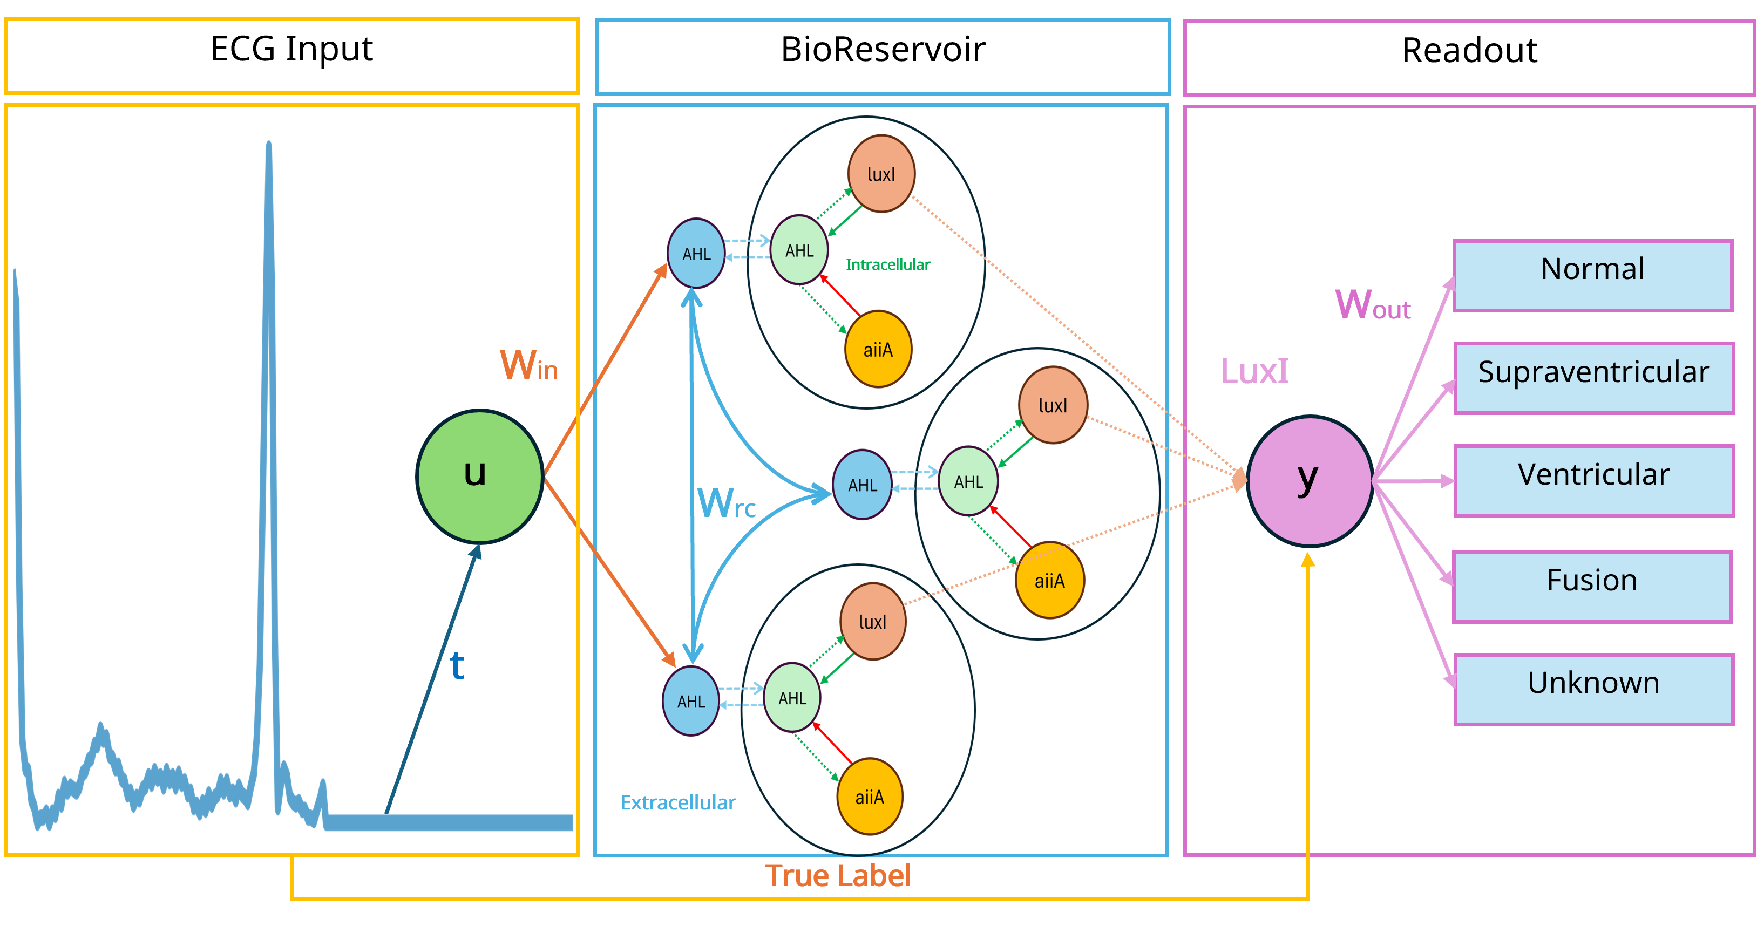
\includegraphics[width=\linewidth]{figures/article/graphical-toc.pdf}
\end{tocentry}

% ---------- References ----------
\bibliography{references}


\end{document}
